% -*- coding: utf-8 -*-

% Ausgabe des Literaturverzeichnisses; ohne weitere Optionen werden nur die
% Bücher und Artikel ausgegeben, die in der Arbeit auch zitiert werden.
\printbibliography

% Anfang des Anhangs
\appendix

% Nicht numeriert, aber trotzdem ins Inhaltsverzeichnis aufgenommen
\addchap{Anhang}

% Abbildungen & Tabellen nicht mehr ins Abbildungs- & Tabellenverzeichnis aufnehmen
\captionsetup[figure]{justification=centering, format=plain, list=no}
\captionsetup[table]{format=plain, list=no}

%\begin{table}
%	\caption{Auswahl der 20 Klassen aus der Oberklasse "CarComponent" für den MVIP-Teildatensatz.}
%	\begin{tabular}{|l|l|l|l|}
%		\hline
%		\textbf{Klasse} & \textbf{Material} & \textbf{Textur} & \textbf{Gebrauchszustand} \\
%		\hline
%		\detokenize{Repstar_RPS_201300} & 'Iron' & 'Metallic', 'Stains' & 'Dirty' \\
%		\detokenize{bosch_0986040600} & 'Iron', 'Plastik' & 'rough', 'hard' & 'Used', 'Old', 'Dirty' \\
%		\detokenize{eiba_5_4} &  &  &  \\
%		\detokenize{cargo_object} & 'Iron' & 'rough', 'hard', 'rubber' & 'Used', 'Old', 'Rusty' \\
%		\detokenize{bosch_1005831623} & 'Iron' & 'rough', 'hard' & 'Used', 'Old', 'Rusty' \\
%		\detokenize{eiba_Denso_9_3} & 'Iron' & 'Metallic', 'Stains' & 'Old' \\
%		\detokenize{bosch_0123100003} & 'Iron', 'Plastik' & 'rough', 'hard' & 'Used', 'Old', 'Dirty' \\
%		\detokenize{casco_cst10287AS} & 'Iron' & 'Metallic' & 'Used' \\
%		\detokenize{Bosch_eiba_9_1} & 'Iron' & 'Metallic', 'rough' & 'Dirty' \\
%		\detokenize{Bosch_BR28_N1} & 'Iron', 'Plastik' & 'Metallic', 'Stains' & 'Dirty' \\
%		\detokenize{vw_ag_03G_903_023_F} & 'Iron', 'Plastik' & 'Metallic', 'rough' & 'Old', 'Used' \\
%		\detokenize{Denso_83631750} & 'Iron', 'copper' & 'Metallic' & 'Used' \\
%		\detokenize{Prestolite_1121} & 'Iron', 'Plastik' & 'Metallic', 'hard' & 'Used' \\
%		\detokenize{eiba_5_16} & 'Iron' & 'Stains', 'hard', 'rough' & 'Dirty', 'Old', 'Rusty', 'Used' \\
%		\detokenize{eiba_9_5} & 'Iron' & 'Metallic' & 'Dirty' \\
%		\detokenize{VW_AG_068911024H} & 'Iron' & 'Metallic', 'smooth' & 'Dirty' \\
%		\detokenize{hellr_8ea_011610411} & 'Iron', 'Plastik' & 'hard', 'rough' & 'Old', 'Rusty', 'Used' \\
%		\detokenize{Hella_8EA_011_610_221} & 'Iron' & 'Metallic', 'Shiny' & 'Used' \\
%		\detokenize{eiba_7_19} & 'Iron' & 'hard', 'rough' & 'Dirty', 'Old', 'Rusty' \\
%		\detokenize{821128} & 'Iron' & 'Metallic', 'Stains' & 'Dirty' \\
%		\hline
%	\end{tabular}
%	\label{app:subdataset}
%\end{table}

\section{Implementierung} \label{sec:app1}

\lstinputlisting[language=python,caption={Begrenzung des Datensatzes auf die 20 "CarComponent" Klassen in der "MVIPDataset"-Klasse.}, label=lst:mvip-classes]{code/code_da-fusion_mvip-class-selection.py}
% \lstinputlisting[language=python,caption={Die verwendeten Text-Prompts zur Generierung der Augmentationen.},label=lst:mvip-prompts]{code/code_da-fusion_prompts.py}

\lstinputlisting[language=python,caption={Funktion zum Laden der Augmentationen in der "MVIPDataset"-Klasse von SupCon.},label=lst:supcon-mvip-parse-augs]{code/code_supcon_mvip-parse-augs.py}
\lstinputlisting[language=python,caption={Vollständige Klasse für die verwendete Verlustfunktion im Supervised Contrastive Learning.},label=lst:supcon-loss]{code/code_supcon_loss.py}

%\lstinputlisting[language=python,caption={Funktion zum Zuschneiden eines Objekts in der "MVIPDataset"-Klasse.},label=lst:da-fusion-crop-object]{code/code_da-fusion_crop-object.py}

%\lstinputlisting[language=python,caption={Python-Skript für die Klasse des MVIP-Teildatensatzes in der Implementierung von DA-Fusion \parencite{Trabucco2024dafusiongithub}.},label=lst:da-fusion-mvip]{../da-fusion/semantic_aug/datasets/mvip.py}
%\lstinputlisting[language=python,caption={Python-Skript für das Textual Inversion Finetuning in DA-Fusion.},label=lst:da-fusion-finetune]{../da-fusion/fine_tune_upstream.py}
%\lstinputlisting[language=python,caption={Python-Skript zum Merging der gelernten Text-Embeddings.},label=lst-da-fusion-aggregate]{../da-fusion/aggregate_embeddings.py}
%\lstinputlisting[language=python,caption={Python-Skript zur Generierung der Augmentationen mit DA-Fusion.},label=lst:da-fusion-generate]{../da-fusion/generate_augmentations.py}

%\lstinputlisting[language=python,caption={Python-Skript für die Klasse des MVIP-Teildatensatzes in der Implementierung von Supervised Contrastive Learning \parencite{Tian2023supcongithub}.},label=lst:supcon-mvip]{../sup-contrast/mvip.py}
%\lstinputlisting[language=python,caption={Python-Skript für die Verlustfunktion in der Implementierung von Supervised Contrastive Learning \parencite{Tian2023supcongithub}.},label=lst:supcon-loss]{../sup-contrast/losses.py}

\newpage

\section{Beispiele für Augmentationen} \label{sec:app2}

\begin{figure}[h]
  \centering
  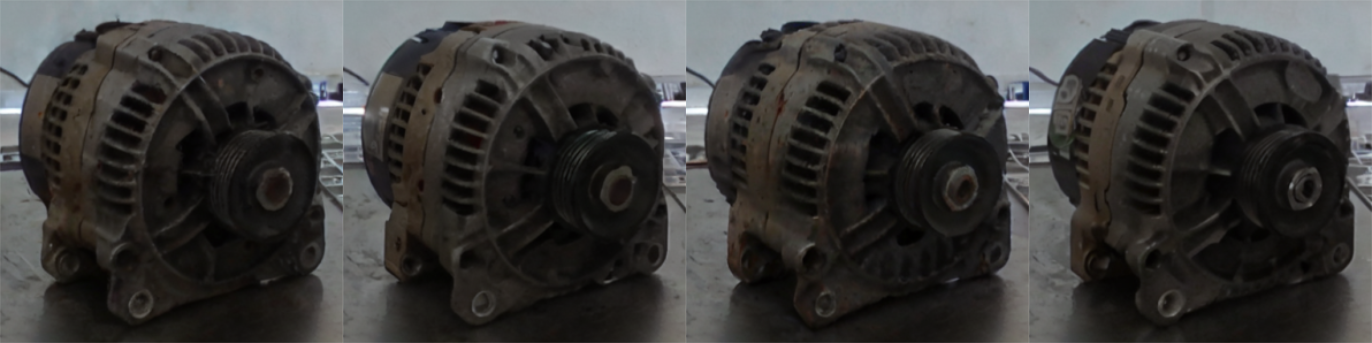
\includegraphics[width=\textwidth]{images/figure_results_id-augs_good_1a.png}
  \caption{Beispiele der In-Distribution-Augmentationen.}
  \label{fig:id-augs-good-1}
\end{figure}

\begin{figure}[h]
  \centering
  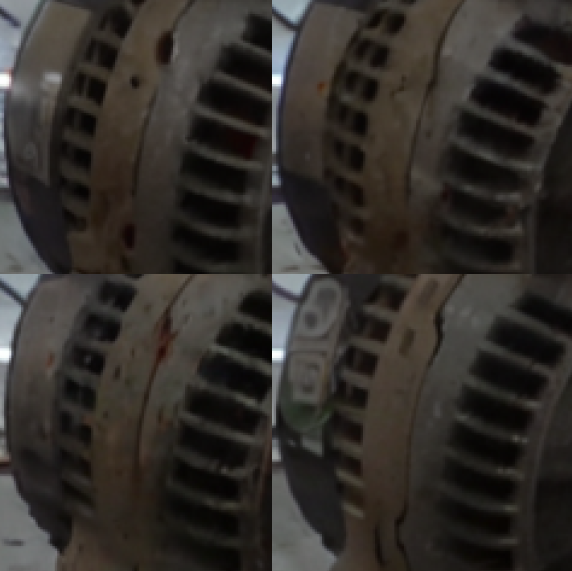
\includegraphics[width=0.48\textwidth]{images/figure_results_id-augs_good_1.png}%
  \hspace{0.02\textwidth}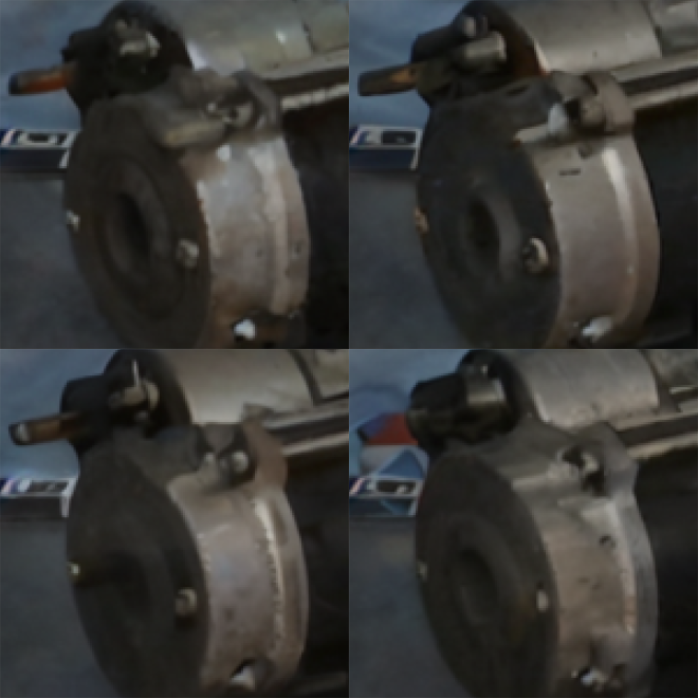
\includegraphics[width=0.48\textwidth]{figure_results_id-augs_good_2.png}%
  \caption{Vergrößerte Ausschnitte von einigen der In-Distribution-Augmentationen.}
  \label{fig:id-augs-good-2}
\end{figure}

\begin{figure}[h]
  \centering
  %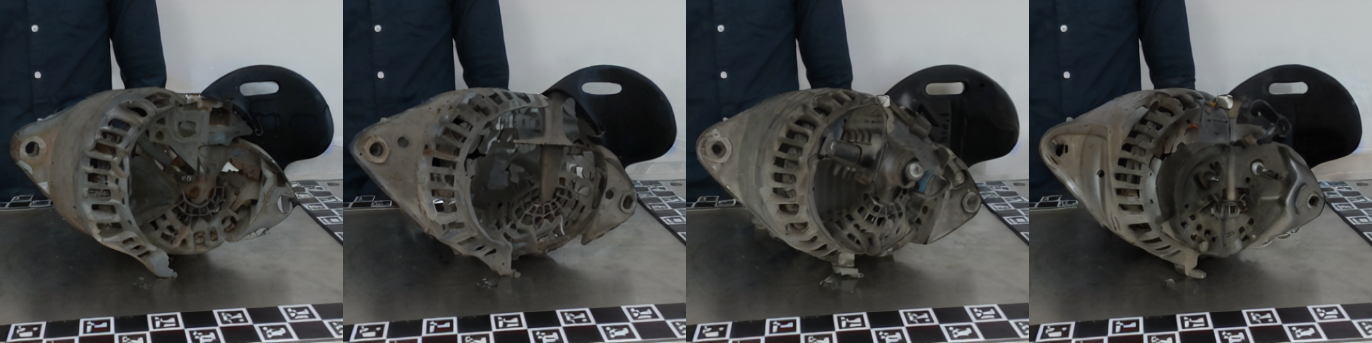
\includegraphics[width=\textwidth]{images/figure_results_id-augs_bad_2a.png}
  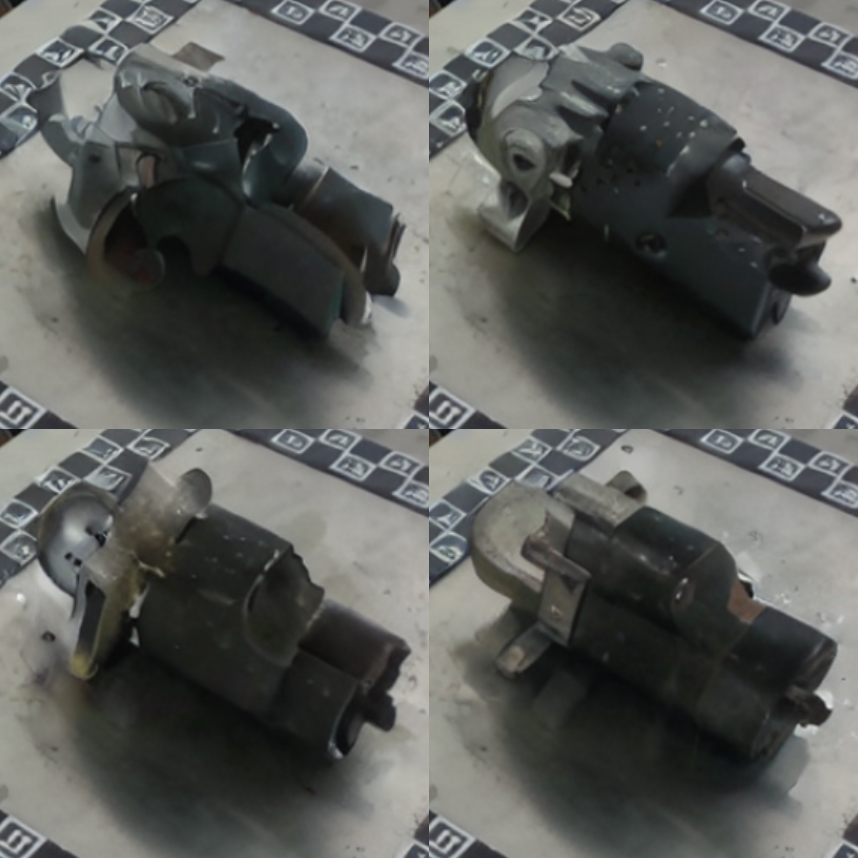
\includegraphics[width=0.48\textwidth]{images/figure_results_id-augs_bad_1.png}%
  \hspace{0.02\textwidth}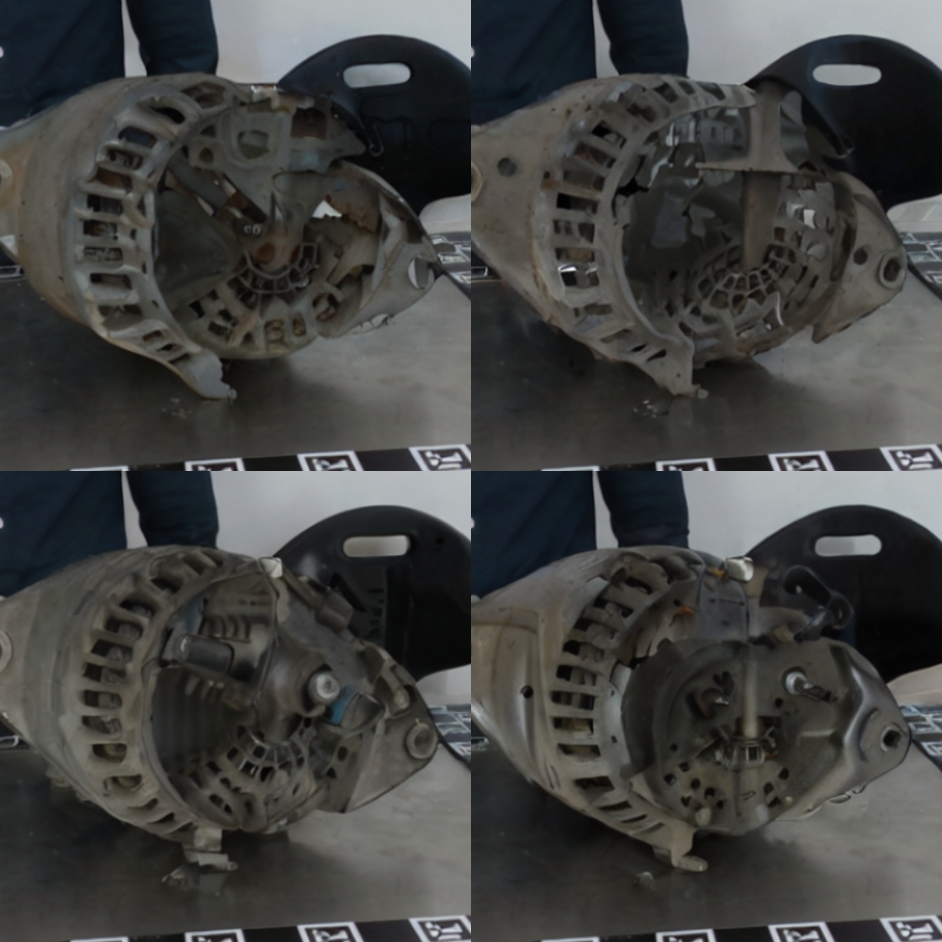
\includegraphics[width=0.48\textwidth]{figure_results_id-augs_bad_2.png}
  \caption{Beispiele für mangelhafte In-Distribution-Augmentationen.}
  \label{fig:id-augs-bad}
\end{figure}

\begin{figure}[h]
  \centering
  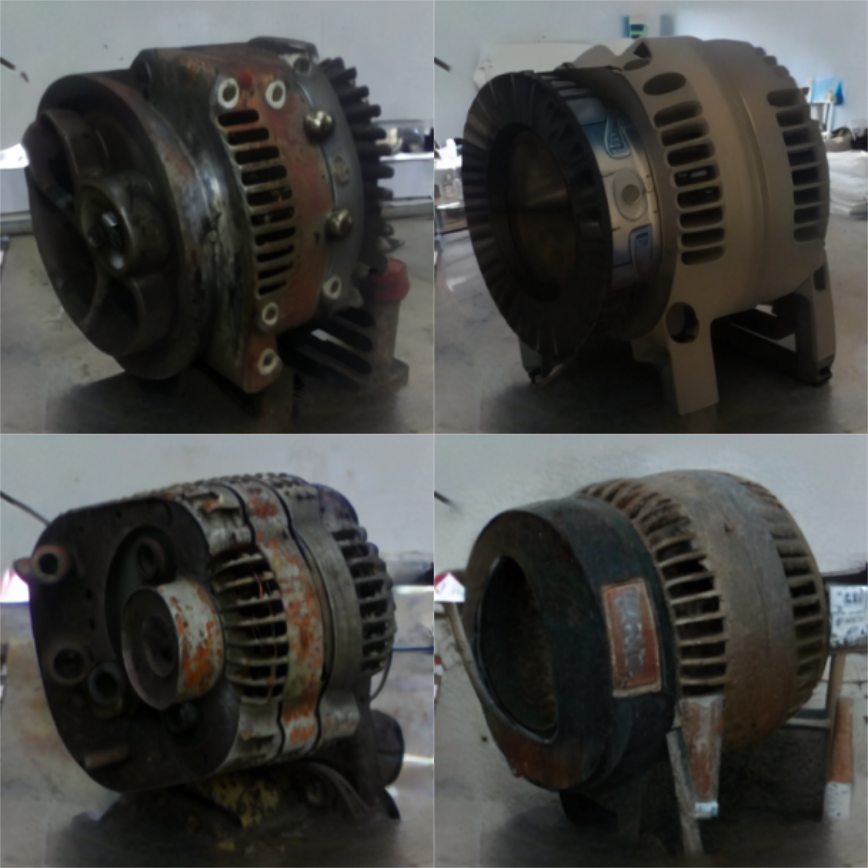
\includegraphics[width=0.48\textwidth]{images/figure_results_ood-augs_good_1.png}%
  \hspace{0.02\textwidth}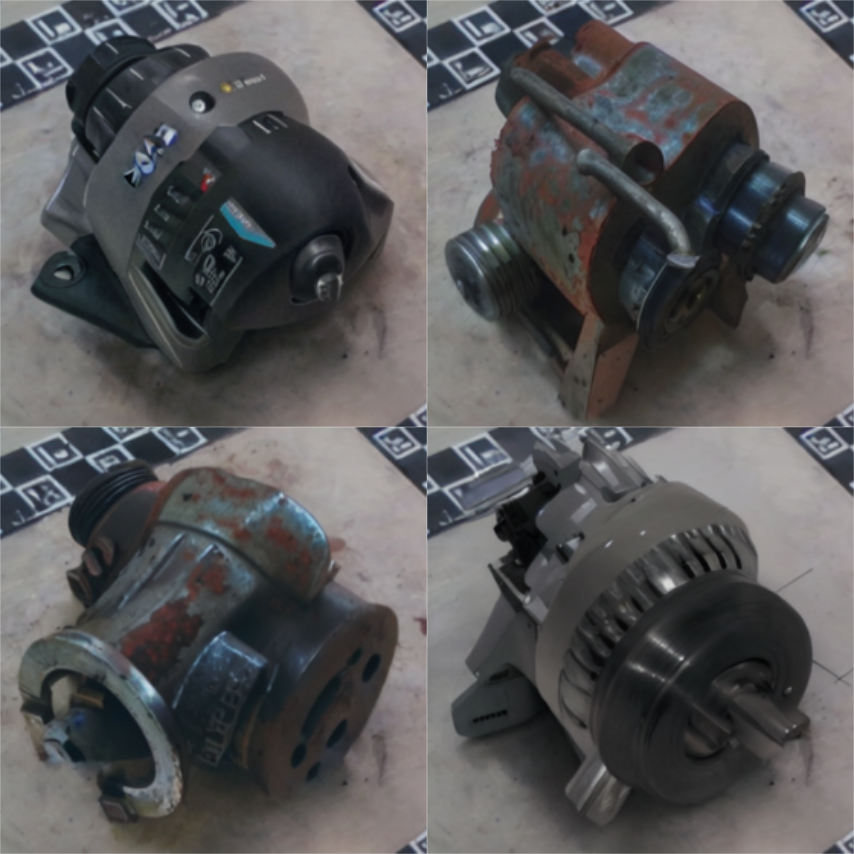
\includegraphics[width=0.48\textwidth]{images/figure_results_ood-augs_good_3.png}\vspace{0.01\textwidth}
  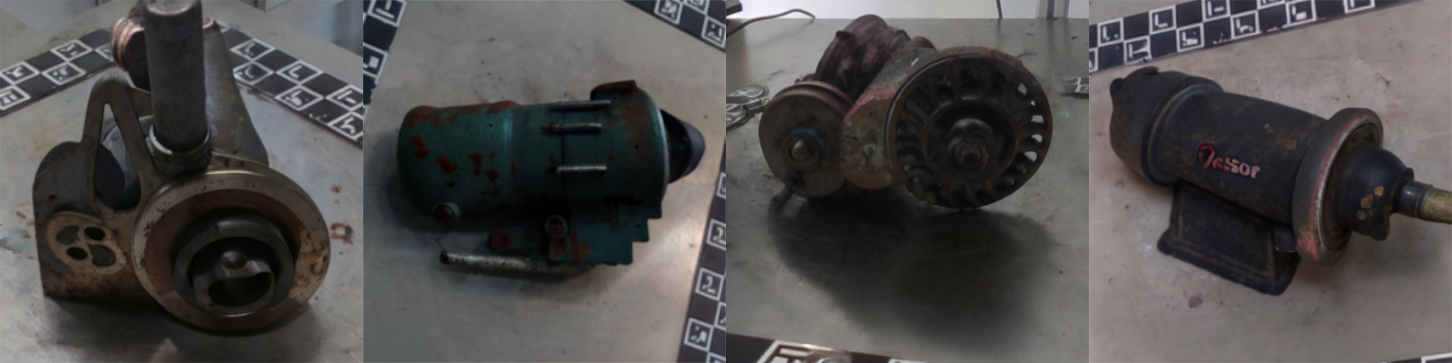
\includegraphics[width=0.98\textwidth]{figure_results_ood-augs_good_4.png}
  \caption{Beispiele der Near Out-of-Distribution-Augmentationen.}
  \label{fig:ood-augs-good}
\end{figure}

\begin{figure}[h]
  \centering
  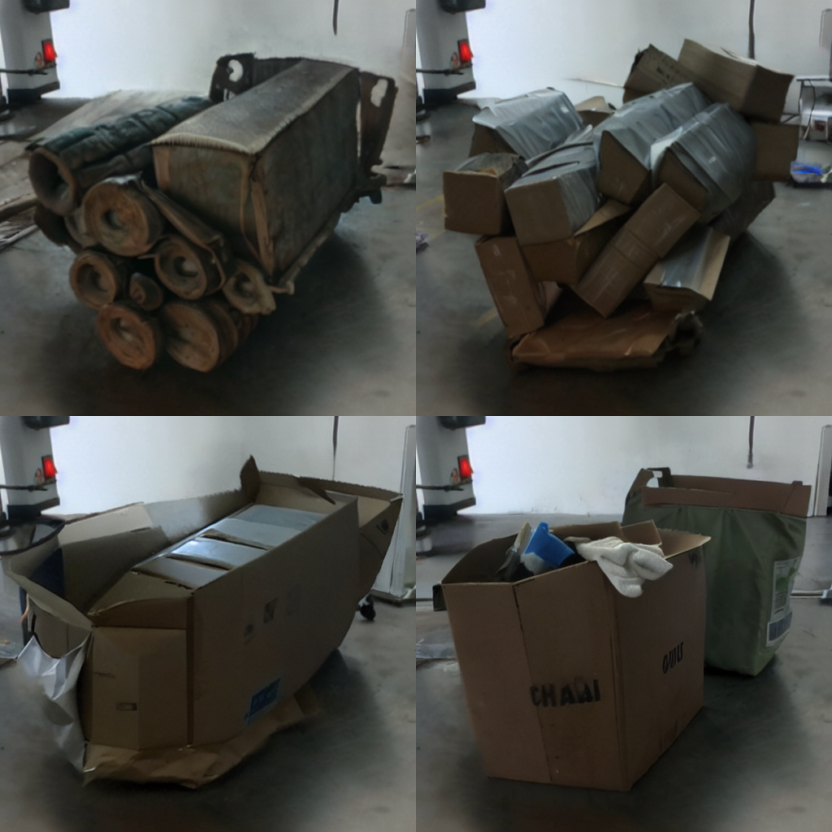
\includegraphics[width=0.48\textwidth]{images/figure_results_ood-augs_bad_1.png}%
  \hspace{0.02\textwidth}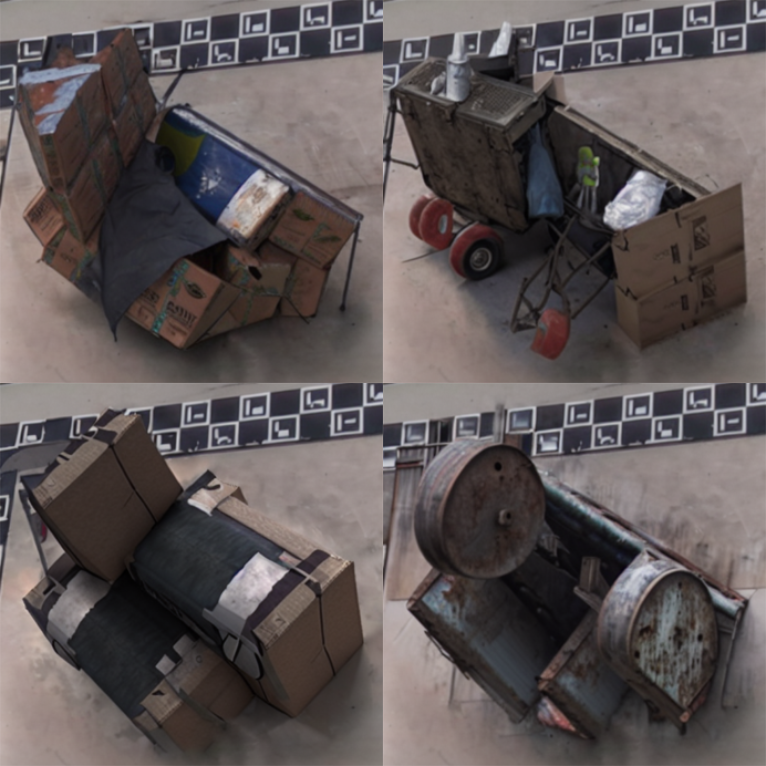
\includegraphics[width=0.48\textwidth]{images/figure_results_ood-augs_bad_2.png}\vspace{0.01\textwidth}
  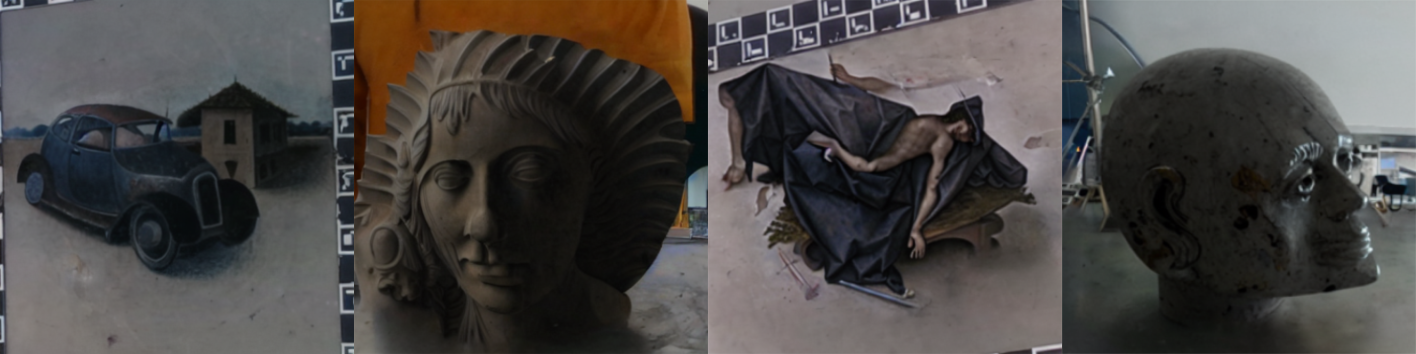
\includegraphics[width=0.98\textwidth]{figure_results_ood-augs_bad_4.png}
  \caption{Beispiele für mangelhafte Out-of-Distribution-Augmentationen.}
  \label{fig:ood-augs-bad}
\end{figure}

\clearpage

% Keine Seitenzahl
\thispagestyle{empty}
% Keine Nummerierung, keine Aufnahme ins Inhaltsverzeichnis
\section*{Eigenständigkeitserklärung}

Hiermit versichere ich, dass ich die vorliegende Bachelorarbeit mit dem Titel
\begin{center}
  \textbf{Contrastive Learning mit Stable Diffusion-basierter Datenaugmentation}
\end{center}
selbstständig und nur mit den angegebenen Hilfsmitteln verfasst habe.  Alle
Passagen, die ich wörtlich aus der Literatur oder aus anderen Quellen wie
z.\,B. Internetseiten übernommen habe, habe ich deutlich als Zitat mit Angabe
der Quelle kenntlich gemacht.

\vspace{2cm}

Hamburg, 23.\ September 2024
